\begin{figure}
	\centering
	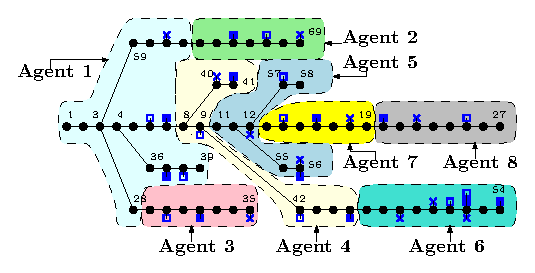
\includegraphics[scale=0.9]{img/top_sim1.eps}
	\caption{The topology of the PG\&E 69-bus distribution system and its 8-agent initial partition \cite{arefifar2012}. Squares indicate the distributed generation units, i.e., \textcolor{blue}{$\blacksquare$} and \textcolor{blue}{$\Box$} represent a renewable generation unit and a dispatchabale generator, respectively, whereas crosses, \textcolor{blue}{$\boldsymbol{\times}$}, indicate the storages.
	}
	\label{fig:cs_top}
\end{figure}
\iffalse 
\begin{table}
	\centering
	\caption{Parameters of the Network Components}
	\label{tab:param}
	\begin{tabular}{c c c c}
		\hline  \noalign{\smallskip}
		\textbf{Parameters} & \textbf{Value} & \textbf{Unit} & \textbf{Bus} \\ 
		\noalign{\smallskip}\hline  \noalign{\smallskip}
		$p^{\mathrm{g,min}}_i$, $p^{\mathrm{g,max}}_i$  & 0, 350 & kW  & $i \in \mathcal{N}^{\mathrm{dg}}$ \\ 		   
		\noalign{\smallskip}
		$x^{\mathrm{min}}_i$, $x^{\mathrm{max}}_i$, $x_{i,0}$ & 30, 100, 50  & \% & $i \in \mathcal{N}^{\mathrm{st}}$\\ 
		\noalign{\smallskip}
		$p^{\mathrm{ch}}_i$, $p^{\mathrm{dh}}_i$ & 100, 100 & kW & $i \in \mathcal{N}^{\mathrm{st}}$  \\ 
		\noalign{\smallskip}
		$e_{\mathrm{cap},i}$ & 1000 & kWh & $i \in \mathcal{N}^{\mathrm{st}}$   \\
		\noalign{\smallskip}
		$a_i$  & 1  & -   & $i \in \mathcal{N}^{\mathrm{st}}$\\
		\noalign{\smallskip}
		$c^{\mathrm{st}}_i$, $c^{\mathrm{g}}_i$  & 1, 10 & -  & $i \in \mathcal{N}$ \\
		\noalign{\smallskip}
		$c^{\mathrm{im}}_i$, $c^{\mathrm{t}}_i$ & 10, 1 & - & $i \in \mathcal{N}$ \\		
		\noalign{\smallskip}
		\hline
	\end{tabular}
\end{table}
\fi 
We consider the PG\&E 69-bus distribution network, as shown in Fig. \ref{fig:cs_top} where dispatchable, solar-based distributed generation, and storage units are added to the network. 
%Moreover,  the available load data are regarded as the maximum loads and the real load profiles and forecasts are generated based on the typical residential and commercial load profiles. The busses that have maximum load greater than 100 kW are considered to have a commercial load profile. Otherwise, they have a residential load profile. 
The simulation time is one day with the sampling time of 15 minutes, implying 96 time steps. Furthermore, the prediction horizon is set to be 8 time steps and the weight on the cost of the repartitioning problem is set as $\alpha=10^4$. %The other parameters of the network components are given in Table \ref{tab:param}. 

%\paragraph*{evolution of partitions formed}
%\paragraph*{evolution of coalitions formed}

The initial partition of the network is based on one of the partitioning results in \cite{arefifar2012}. How the microgrids form coalitions throughout the simulation can be seen in Figure \ref{fig:co_res}. %At $k=1,\dots,13$, all microgrids obtained from the initial partition of the network are still self-sufficient. Then, at $k=14$, for the first time the network must be repartitioned. Moreover, for $k=14,\dots,24$, the repartitioning and coalition formation procedures are always performed. During this period, two microgrids are not self-sufficient and join together as a coalition. At $k=25$, the repartitioning procedure produces self-sufficient microgrids, %as shown in Figure \ref{fig:part_res}.a, 
%and self-sufficiency is maintained until $k=57$. 
We can observe that 
 during the peak hours $57\leq k \leq 80$, coalitions must be formed and, even at a certain period, all microgrids must join as one coalition, whereas during the off-peak hours, self-sufficient microgrids can be formed. % We can also see gradual changes of the coalitions formed particularly at $k\geq57$. Moreover, towards the end of the simulation we can also see that by performing repartitioning of the network, the number of self-sufficient microgrids improves as the number of distinct coalitions also increases. Finally, at $k=96$, all the microgrids formed are self-sufficient, %as shown in Figure \ref{fig:part_res}.b. %In addition, one can compare the differences between the initial partition in Figure \ref{fig:cs_top} and the resulting partitions in Figure \ref{fig:part_res}.
%\paragraph*{suboptimality} 
Figure \ref{fig:deltaJ} shows the stage costs for all time steps and the sub-optimality of the proposed scheme. %As provided by Proposition \ref{prop:est_difJ}, the scheme might also compute an upper bound of the sub-optimality, which is shown by the dashed line in the bottom plot of Figure \ref{fig:deltaJ}. %The average sub-optimality throughout the simulation is $21.93\%$, whereas the average upper bound of the sub-optimality defined in Proposition \ref{prop:est_difJ} is $51.38\%$. %Furthermore, during $k=62,\dots,72$, when all microgrids form one coalition, the optimal cost values are obtained since a fully distributed scheme is employed.
\color{black}

\begin{figure}
	\centering
	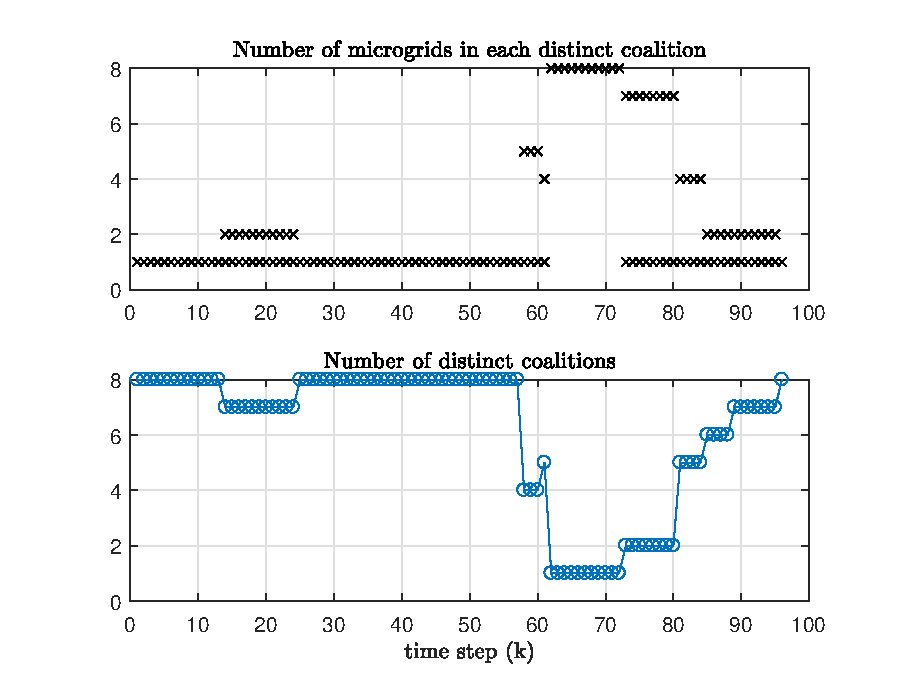
\includegraphics[scale=0.6]{img/co_res.eps}
	\caption{The evolution of coalitions formed.
	}
	\label{fig:co_res}
\end{figure}
\iffalse 
\begin{figure}
	\centering
	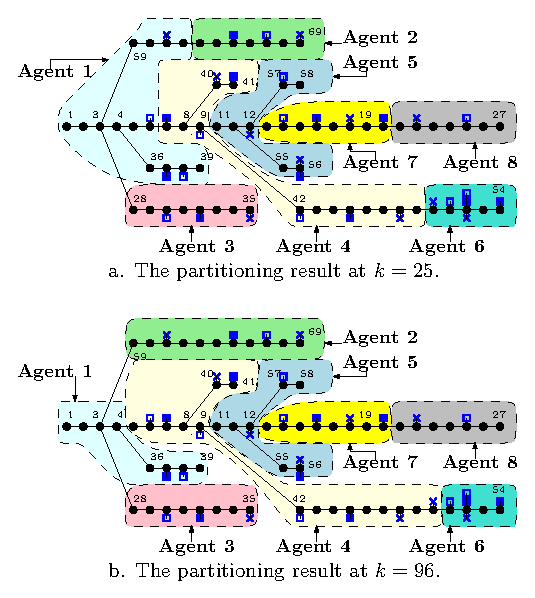
\includegraphics[scale=0.9]{img/part_res.eps}
	\caption{Partitioning results at a. $k=25$ and b. $k=96$. At both time instants, the resulting microgrids are self-sufficient.
	}
	\label{fig:part_res}
\end{figure}
\fi 
\begin{figure}
	\centering
	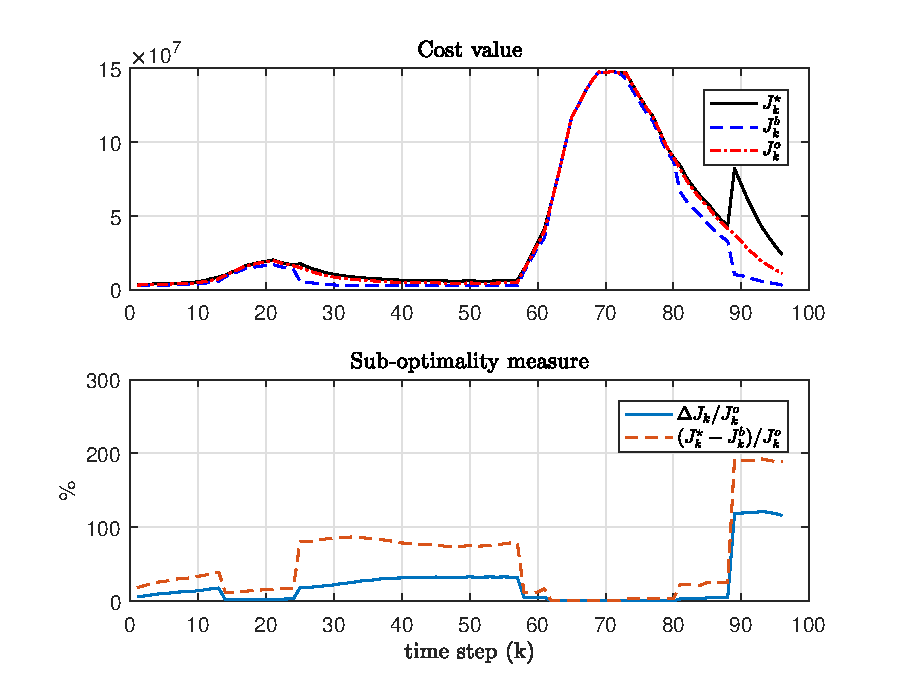
\includegraphics[scale=0.6]{img/delta_J2.eps}
	\caption{Top plot shows the cost values computed using the proposed scheme, $J^{\star}_k$, (solid line), by solving Problem \eqref{eq:MPC_net} centrally as the benchmark $J^{o}_k$, (dashed-dotted line), and the lower bound, $J^{b}_k$ (dashed line). Bottom plot shows the suboptimality of the proposed scheme and its upper bound.
	}
	\label{fig:deltaJ}
\end{figure}